\documentclass[conference,10pt]{IEEEtran}
\usepackage[T1]{fontenc}
\usepackage{amsmath,amssymb,amsthm,booktabs,array,microtype}
\usepackage[hidelinks]{hyperref}
\usepackage{placeins,balance,needspace,etoolbox}
\newcommand{\DoNotLoadEpstopdf}{}
\usepackage{tikz}
\usetikzlibrary{arrows.meta,positioning}
\definecolor{sourceblue}{RGB}{29,83,135}
\definecolor{fliporange}{RGB}{166,76,0}
\definecolor{softblue}{RGB}{237,244,250}
\definecolor{softorange}{RGB}{255,244,232}
\newcommand{\G}{\mathsf{G}}\newcommand{\F}{\mathsf{F}}
\newcommand{\CPre}{\operatorname{CPre}}\newcommand{\Pref}{\operatorname{Pref}}
\newcommand{\EPre}{\operatorname{EPre}}\newcommand{\code}[1]{\texttt{#1}}
\newtheorem{theorem}{Theorem}\newtheorem{proposition}[theorem]{Proposition}
\newtheorem{corollary}[theorem]{Corollary}\newtheorem{lemma}[theorem]{Lemma}
\BeforeBeginEnvironment{corollary}{\Needspace{13\baselineskip}}
\newcolumntype{L}[1]{>{\raggedright\arraybackslash}p{#1}}
\title{Auditing Controller Replacement after Environment-Model Change}
\author{\IEEEauthorblockN{Anonymous authors}}
\begin{document}\raggedbottom\maketitle
\begin{abstract}
After an environment-model change, a replacement controller may need to
continue from the current state with pending obligations. We audit when a
negative translated synthesis answer can justify excluding such a continuation.
For the one-way Boolean-helper encoding used in Kind synthesis, we characterize
exactly which strict-winning source continuations survive. The helper input can
release environment safety one step before controller safety. With guards covering all safety duties, a continuation survives exactly when
one winning source strategy keeps a safe response to the helper's first
change available for as long as the helper may wait.
This yields a necessary and sufficient whole-region preservation condition
and an extension for retained safety duties. A constructed Patrol update
shows why responding safely now is insufficient: fulfilling a charging
obligation can destroy that response option. Separate Vehicle and Obstacle
analyses distinguish initialization, continuation preservation and tool answers.
At a fixed Obstacle query, releasing only the first-change system duty changes
the same cooperative raw solver's answer from false to true. Executable case checks make the
audit inspectable. The results support candidate-exclusion reasoning;
general installation guarantees and operational benefit remain outside the established scope.
\end{abstract}
\begin{IEEEkeywords}
self-adaptive systems, reactive synthesis, continuation preservation,
controller replacement, verification artifacts
\end{IEEEkeywords}
\section{Introduction}\label{sec:intro}
A patrol robot still owes a charging visit when its environment model
changes. A replacement controller would inherit its position and the monitor
recording that request. Before excluding candidate requirements or arranging
a controller update~\cite{specrepair,degradation,dupdate}, an adaptation
manager therefore asks: \emph{can a controller still meet these requirements
from the retained state?} We audit when a negative translated synthesis
answer justifies excluding that continuation. This is the candidate-exclusion
decision in replacement planning.

Reactive synthesis asks for a controller that responds to environment
inputs. GR(1) specifications combine initial conditions, safety rules and
recurring goals for the environment and controller. Under \emph{strict}
semantics, the controller owes safety on every prefix that respects ENV
initialization and safety; later unfairness cannot excuse an earlier unsafe
response. Kind adds cooperation to strict winning: after every history the
strategy induces, even after an environment violation, that same strategy
at its reached memory must permit a safe, fair environment future. We call
this property \emph{source-kind} when it holds before translation; its full
definition appears in Section~\ref{sec:source-kind}.

We call the requirements before translation the \emph{source}; after an
update, these are the candidate's updated requirements. Figure~\ref{fig:overview}
separates the source question from the translated game and the procedure
answering it. A raw call invokes the underlying solver, whereas a public
action also selects a translation and solver path. Preservation and
query/objective correspondence are separate obligations in this picture.
% Conceptual reasoning for a retained-state query; not an implemented pipeline.
\begin{figure}[!t]
\centering
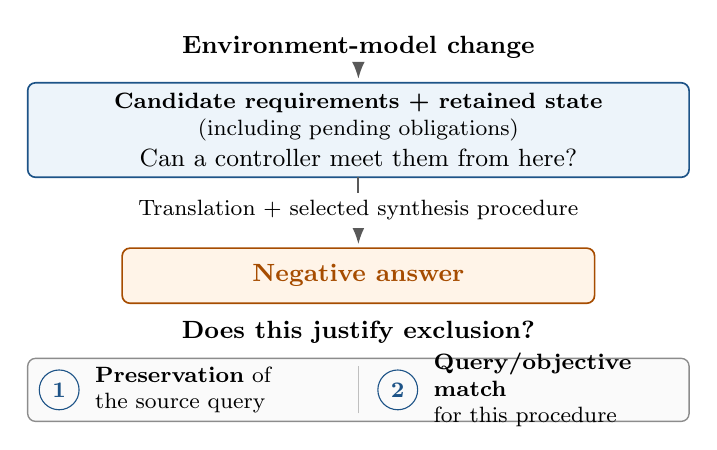
\begin{tikzpicture}[x=1mm,y=1mm,>=Latex,
 every node/.style={font=\footnotesize,align=center,inner sep=.5mm}]
\path[use as bounding box] (0,0) rectangle (84,50);
% The change motivates the concrete continuation question below.
\node[font=\small\bfseries] at (42,47.5) {Environment-model change};
\draw[->,black!65,line width=.7pt] (42,45.1) -- (42,43.5);
\draw[sourceblue,fill=softblue,line width=.6pt,rounded corners=1mm]
  (0,31) rectangle (84,43);
\node[font=\footnotesize\bfseries] at (42,40.5)
  {Candidate requirements + retained state};
\node at (42,37) {(including pending obligations)};
\node[font=\small] at (42,33.5)
  {Can a controller meet them from here?};
% A negative translated answer leaves the exclusion inference to be checked.
\draw[->,black!65,line width=.7pt] (42,31) -- (42,22.5);
\node[fill=white,inner sep=1mm] at (42,26.8)
  {Translation + selected synthesis procedure};
\draw[fliporange,fill=softorange,line width=.6pt,rounded corners=1mm]
  (12,15) rectangle (72,22);
\node[font=\small\bfseries,text=fliporange] at (42,18.5) {Negative answer};
\node[font=\small\bfseries] at (42,11.3) {Does this justify exclusion?};
% Both obligations are necessary to use this answer to discard a continuation.
\draw[draw=black!45,fill=black!2,line width=.5pt,rounded corners=1mm]
  (0,0) rectangle (84,8);
\draw[black!25,line width=.4pt] (42,1) -- (42,7);
\node[circle,draw=sourceblue,text=sourceblue,font=\footnotesize\bfseries,
  inner sep=.9mm] at (4,4) {1};
\node[anchor=west,align=left,text width=32mm] at (8,4)
  {\textbf{Preservation} of\\the source query};
\node[circle,draw=sourceblue,text=sourceblue,font=\footnotesize\bfseries,
  inner sep=.9mm] at (47,4) {2};
\node[anchor=west,align=left,text width=29mm] at (51,4)
  {\textbf{Query/objective match}\\for this procedure};
\end{tikzpicture}
\caption{Reasoning about a retained-state continuation during replacement
planning. A translated negative supports exclusion only after checking
preservation of the queried source property and agreement between the
procedure, query and objective. This is a reasoning diagram, not an
implemented pipeline.}
\label{fig:overview}
\end{figure}


The helper is an environment-controlled Boolean input that can change
permanently from false to true. Its first change releases ENV safety one
edge before SYS safety, so the controller must still answer safely on that edge.

Patrol exposes why this timing matters. At the retained state the robot can
answer every input allowed by the first helper change. Yet meeting its
charging obligation lets the environment steer it into a conflict: remain
at the charger and avoid a blocked checkpoint placed there. That placement
is forbidden by the source but permitted by the helper. Thus being able to
respond now differs from maintaining that ability while winning.

An existing complete-relation correction releases both duties on the
first-change edge and preserves the whole source strict-winning
region~\cite{spectrarelease2024}. Our question is which continuations survive
the original printed encoding, including exports that retain auxiliary
duties; correcting the encoding does not characterize those survivors.
The public Kind path inspected for the Obstacle inputs also uses a syntactic
reduction and raw solver separately from that correction
(Section~\ref{sec:evidence}). We give exact preservation conditions and a
local intervention on that solver query, rather than a new solver or
correction. With complete safety-relation guards, the central condition is that one winning source strategy keep
a safe first-change response available for as long as the helper may wait.
We make three contributions:
\begin{enumerate}
\item \emph{Exact preservation for exclusion.} We characterize the surviving strict-winning
continuations, derive a necessary and sufficient whole-region condition,
and extend the result to safety duties retained after the change. All three
results have complete proofs in the main paper.
\item \emph{Constructive and implementation-bound evidence.} A constructed
ENV-only Patrol update separates responding now from maintaining that ability
while winning. Vehicle separates initialization from continuation preservation.
At a fixed Obstacle requirements-replacement query, releasing only the
first-change SYS duty changes the same solver's
answer from false to true.
\item \emph{An exclusion contract and executable checks.} We connect
query/objective correspondence and preservation to candidate exclusion.
The accompanying release binds typed model snapshots to positive
witnesses, loss certificates and saved evidence for Vehicle, Patrol and
Obstacle B~\cite{artifactrepository}.
\end{enumerate}
We first explain the Patrol challenge, give the basic strict result, then
close Patrol's positive and negative arguments before treating retained duties.
The cases then connect preservation to tool answers, before the
candidate-exclusion audit and common limits.

\section{A Continuation That Should Not Be Discarded}
\label{sec:motivation}
Consider a robot that repeatedly visits three checkpoints and a charger on a
$5\times5$ grid. Charging requires a dwell period, and a request monitor
records whether a charging visit is owed. These duties come from the public
Patrolling specification, corpus~277~\cite{kindartifact}. We use its unchanged
source as the new model and construct an old model that additionally fixes
the displayed layout and keeps all checkpoints open. Removing those old ENV
restrictions leaves system requirements, types and monitors unchanged.
Checkpoint positions still remain fixed from one round to the next, but a
distant checkpoint may now close. This update scenario and reuse policy
were constructed after diagnosis.

\subsection{The retained entry and two safety rules}
An allowed old-model step reaches entry $r$: the robot is at the origin
$O=(0,0)$, all checkpoints are open, charging is unavailable, the dwell
counter $c$ is zero and the charging request is pending. Its retained route phase
is ready to visit checkpoint $A$. The checkpoints are at
$(0,4),(2,4),(4,4)$ and the charger at $H=(4,0)$
(Fig.~\ref{fig:patrol-grid}).
% Legal source-policy route only. No off-assumption completion is depicted.
% Uses the main document's TikZ, arrows.meta, sourceblue/fliporange colors.
\begin{figure}[!ht]
\centering
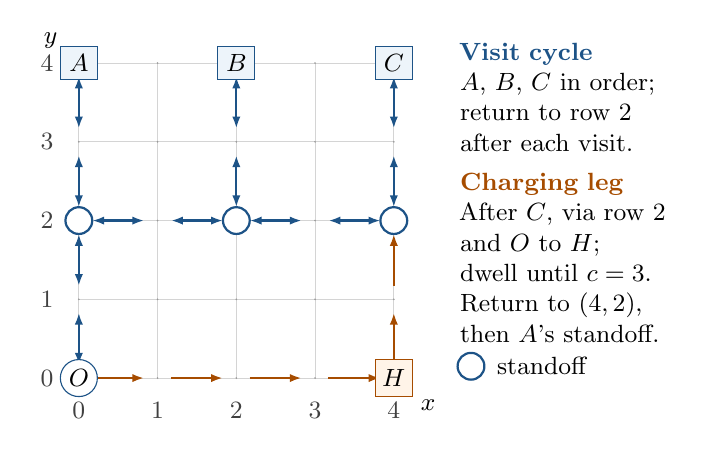
\begin{tikzpicture}[
 x=10mm,y=10mm,
 >={Latex[length=1.5mm,width=1.05mm]},
 every node/.style={font=\small,inner sep=1pt},
 patrol/.style={sourceblue,line width=.8pt,<->,shorten <=1.7mm,shorten >=1.7mm},
 charge/.style={fliporange,line width=.9pt,->,shorten <=1.7mm,shorten >=1.7mm},
 checkpoint/.style={draw=sourceblue,fill=softblue,rectangle,
   minimum width=4.7mm,minimum height=4.2mm,font=\small\bfseries},
 standoff/.style={draw=sourceblue,fill=white,circle,
   line width=.8pt,minimum size=3.4mm,inner sep=0pt}
]
\path[use as bounding box] (-.65,-.65) rectangle (7.85,4.45);

% The grid points, not diagonals or geometric shortcuts, are the source states.
\draw[step=1,black!17,line width=.3pt] (0,0) grid (4,4);
\foreach \x in {0,...,4} {
  \foreach \y in {0,...,4} {
    \fill[black!40] (\x,\y) circle[radius=.35pt];
  }
  \node[anchor=north,text=black!75] at (\x,-.27) {$\x$};
}
\foreach \y in {0,...,4} {
  \node[anchor=east,text=black!75] at (-.28,\y) {$\y$};
}
\node[anchor=west] at (4.30,-.35) {$x$};
\node[anchor=south] at (-.36,4.15) {$y$};

% O to the first standoff, and the return to O after the checkpoint visits.
\foreach \y in {0,1} {
  \draw[patrol] (0,\y)--(0,{\y+1});
}
% Row 2 connects the standoffs; these edges are reused on return journeys.
\foreach \x in {0,1,2,3} {
  \draw[patrol] (\x,2)--({\x+1},2);
}
% Each visit approaches through row 3 and retreats along the same unit edges.
\foreach \x in {0,2,4} {
  \foreach \y in {2,3} {
    \draw[patrol] (\x,\y)--(\x,{\y+1});
  }
}
% Charging: O along row 0 to H; after dwelling, H to (4,1) to (4,2).
\foreach \x in {0,1,2,3} {
  \draw[charge] (\x,0)--({\x+1},0);
}
\foreach \y in {0,1} {
  \draw[charge] (4,\y)--(4,{\y+1});
}

\foreach \x in {0,2,4} {\node[standoff] at (\x,2) {};}
\node[checkpoint] at (0,4) {$A$};
\node[checkpoint] at (2,4) {$B$};
\node[checkpoint] at (4,4) {$C$};
\node[draw=sourceblue,fill=white,circle,minimum size=4.7mm] at (0,0) {$O$};
\node[draw=fliporange,fill=softorange,rectangle,minimum size=4.7mm] at (4,0) {$H$};

\node[anchor=north west,align=left,text width=29mm] at (4.80,4.30)
 {\textcolor{sourceblue}{\textbf{Visit cycle}}\\
 $A$, $B$, $C$ in order;\\
 return to row 2\\
 after each visit.\\[3pt]
 \textcolor{fliporange}{\textbf{Charging leg}}\\
 After $C$, via row 2\\
 and $O$ to $H$;\\
 dwell until $c=3$.\\
 Return to $(4,2)$,\\
 then $A$'s standoff.};
\node[standoff] at (4.98,.15) {};
\node[anchor=west] at (5.27,.15) {standoff};
\end{tikzpicture}
\caption{Patrol's legal source route uses unit cardinal moves.
Before each checkpoint visit, wait at its circled standoff while the next
blocked flag $d_i'$ is true; otherwise approach, visit and retreat.
The charging leg restarts the visit cycle.}
\label{fig:patrol-grid}
\end{figure}


Write $p$ for the robot position and $z$ for charging availability; primes denote next values. A checkpoint $i$ has
blocked flag $d_i$ and position $t_i$. Two SYS safety duties will conflict:
\begin{equation}
\begin{aligned}
\text{Dwell:}\quad &(p=H\land c<3)\Rightarrow p'=H,\\
\text{Avoidance:}\quad &d_i\Rightarrow p'\ne t_i'.
\end{aligned}
\label{eq:patrol-conflict}
\end{equation}
Avoidance combines the \emph{current} blocked flag with the \emph{next}
checkpoint position. Source-legal inputs keep positions fixed and cannot
change a flag while the robot is within one cell of that checkpoint.
The complete ENV justice list requires only that each of the three
checkpoints reopen infinitely often. There is \emph{no charging-availability
justice}: availability is governed by the safety rule $c=3\Rightarrow z'$,
using the current counter.

\subsection{Responding now is not enough}
At $r$, staying at $O$ is safe even for an arbitrary typed next input:
the robot is not dwelling and every current blocked flag is false.
It also has a source policy that visits the checkpoints, waits for reopening
when needed, and charges repeatedly; Section~\ref{sec:patrol} proves this
using the displayed route.

The helper encoding adds an internal ENV Boolean $b$, initially false,
that can change to true once. This is a game input, not the physical update.
Table~\ref{tab:timing} shows the challenge: the first change releases ENV
safety immediately while SYS still owes one safe response. The strict
meaning of that duty is defined in Section~\ref{sec:formal}.
\begin{table}[!ht]
\caption{One edge separates the releases for the complete literal relations
in Eq.~\eqref{hpb:literal}. ``Any typed'' includes source-forbidden inputs.
The last column uses the existing corrected guard.}
\label{tab:timing}\centering\small
\begin{tabular}{@{}llll@{}}\toprule
Helper & Legal ENV input & SYS duty & Corrected duty\\\midrule
$0\to0$ & Source-legal & Source & Source\\
$0\to1$ & Any typed & Source & None\\
$1\to1$ & Any typed & None & None\\\bottomrule
\end{tabular}
\end{table}


Table~\ref{tab:patrol-entry} shows how a legal source prefix reaches the
point where that response fails.
ENV keeps the checkpoints open and charging unavailable until the first
arrival at $H$, then legally closes distant checkpoint $A$ on the next round.
\begin{table}[!ht]
\caption{Milestones of Patrol's legal prefix. Reaching $H$ may take
several rounds; the next row is one dwell edge later. At $x$ the request
has cleared but the dwell is unfinished.}
\label{tab:patrol-entry}\centering\small
\begin{tabular}{@{}L{32mm}ccL{23mm}@{}}\toprule
State / event & $p$ & $c$ & Request\\\midrule
Retained entry $r$ & $O$ & 0 & pending\\
First arrival at $H$ & $H$ & 0 & pending\\
Next legal dwell; $A$ closes ($x$) & $H$ & 1 & cleared (idle)\\\bottomrule
\end{tabular}
\end{table}

Clearing the request records the visit; it does not finish the dwell duty,
which remains active until the counter reaches three. From $x$, a first-change input places the already blocked checkpoint at
$H$: Dwell requires the robot to stay there and Avoidance forbids it.
That input belongs to the translated game; moving a checkpoint is not
source-legal. A different safe strategy cannot avoid the issue: never
reaching $H$ leaves the request pending forever, whereas first reaching
$H$ permits the same legal next round and conflict
(Fig.~\ref{fig:patrol-motivation}). The proof will cover every safe strategy.
The question is whether a winning policy can \emph{keep} a response available,
not only whether the retained state has one now.
\begin{figure}[!ht]
\centering
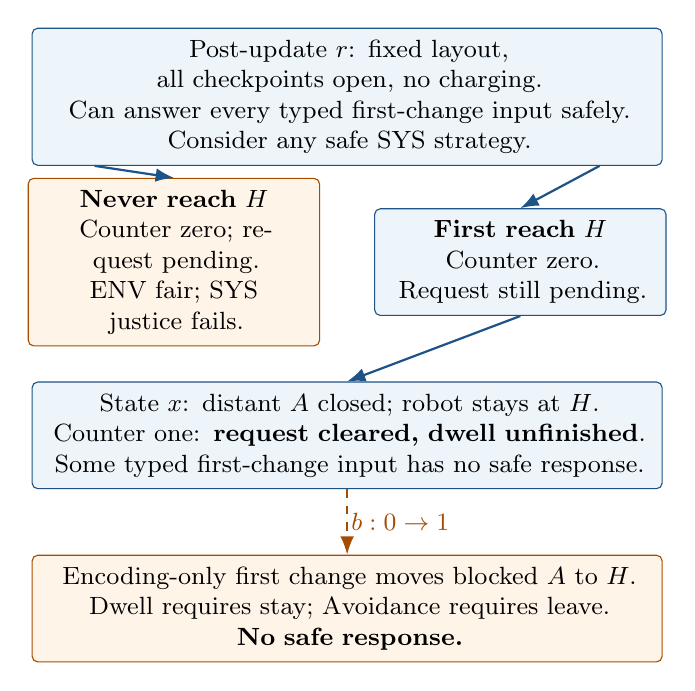
\begin{tikzpicture}[>=Latex,x=1mm,y=1mm,
every node/.style={font=\small,align=center,inner sep=1.5mm},
wide/.style={draw=sourceblue,fill=softblue,rounded corners=2pt,text width=77mm},
branch/.style={draw,rounded corners=2pt,text width=34mm},
phase/.style={fill=white,inner sep=.4mm}]
\node[wide] (start) at (42,72)
 {Post-update $r$: fixed layout,\\all checkpoints open, no charging.\\
 Can answer every typed first-change input safely.\\
 Consider any safe SYS strategy.};
\node[branch,draw=fliporange,fill=softorange] (never) at (20,51)
 {\textbf{Never reach $H$}\\Counter zero; request pending.\\ENV fair; SYS justice fails.};
\node[branch,draw=sourceblue,fill=softblue] (reach) at (64,51)
 {\textbf{First reach $H$}\\Counter zero.\\Request still pending.};
\draw[->,thick,sourceblue] (start.south west)++(8,0)--(never.north);
\draw[->,thick,sourceblue] (start.south east)++(-8,0)--(reach.north);
\node[wide] (closed) at (42,29)
 {State $x$: distant $A$ closed; robot stays at $H$.\\
 Counter one: \textbf{request cleared, dwell unfinished}.\\
 Some typed first-change input has no safe response.};
\draw[->,thick,sourceblue] (reach.south)--(closed.north);
\node[wide,draw=fliporange,fill=softorange] (flip) at (42,7)
 {Encoding-only first change moves blocked $A$ to $H$.\\
 Dwell requires stay; Avoidance requires leave.\\\textbf{No safe response.}};
\draw[->,thick,fliporange,dashed] (closed.south)
 --node[phase,right] {$b:0\to1$} (flip.north);
\end{tikzpicture}
\caption{All-response loss from Patrol's source-winning entry. Solid arrows use source-legal inputs
while $b=0$. The dashed first-change edge follows the legal edge that
clears the request. The two branches cover every safe strategy.}
\label{fig:patrol-motivation}
\end{figure}


\FloatBarrier
\section{What the Encoding Preserves}\label{sec:formal}
\subsection{The game and the meaning of a continuation}\label{sec:semantics}
A finite, fully observed Mealy game has nonempty typed input and response
carriers $E,Y$ and states $s=(e,y)\in D=E\times Y$, including all logical
monitors. In one round ENV chooses $e'$; SYS observes it and chooses $y'$,
reaching $s'=(e',y')$. ENV safety $\rho_e(s,e')$ is independent of the next
SYS response. SYS safety $\rho_s(s,e',y')$ includes every system constraint
and monitor update. A typed input is in its declared domain; a
\emph{source-legal} input also satisfies $\rho_e$. Neither safety relation
need be total. Invalid type encodings are outside $D$.

The ENV and SYS justice lists define generalized B\"uchi objectives $A,G$:
each listed predicate must hold infinitely often. Under \emph{strict}
semantics~\cite{gr1,kind}, when ENV initialization holds, SYS owes its
initializer and safety on every edge whose entire ENV-safety prefix,
including that edge, is legal. An actual ENV safety violation releases the safety duty on the violating
edge and thereafter. On infinite plays satisfying
ENV initialization and safety, SYS must satisfy $A\Rightarrow G$.
Future ENV unfairness cannot excuse an earlier required safety violation.
Strategies may use history and private memory and supply typed responses
even after ENV violations.

Let $W$ be the set of states from which SYS has a strict-winning source
continuation. Such an \emph{active} entry has met ENV initialization, prior
ENV safety and the required SYS duties. Membership in $W$ says neither that
the state is reachable nor that it is an allowed initializer; ENV dead ends
may win vacuously. Initial synthesis instead asks whether \emph{each} allowed
ENV initial value admits \emph{some} allowed SYS response in the winning
region. A retained-state query fixes both components, including the pending
obligations. It cannot select a different initial response. These distinct
questions will matter in Vehicle and Obstacle.

\subsection{The first-change edge}
The helper $b$ starts false, is offered with the next ENV input and is
observed before SYS responds. It can become true only once. Kind's printed
clause guards relax ENV safety with the \emph{next} helper and SYS safety
with the \emph{current} helper~\cite[Sec.~4.1]{kind}. When these guards cover
the \emph{complete} safety relations, including all auxiliaries, the encoded
relations and objectives are
\begin{equation}
\begin{aligned}
\rho_e^R&=(\rho_e\lor b')\land(\neg b\lor b'),&
\rho_s^R&=\rho_s\lor b,\\
A^R&=A\land\G\F\neg b,&G^R&=G.
\end{aligned}\label{hpb:literal}
\end{equation}
Initialization is unchanged except that ENV also fixes $b=0$.
The factor $\neg b\lor b'$ makes the change one-way. ``Complete'' describes
the guards' coverage, not whether a safe response exists.


Table~\ref{tab:timing} showed the timing consequence: on the first-change
edge, ENV has already been released but SYS has not. The added ENV justice $\G\F\neg b$ becomes
impossible after a permanent change to true. Strict semantics nevertheless
requires the safe response on that legal edge: future unfairness does not
waive present safety.

The existing correction uses
$\rho_s^{R^+}=\rho_s\lor b\lor b'$~\cite{spectrarelease2024}.
It releases the first-change duty and preserves the source strict region
(Supplement~L.6). The theorem below characterizes the encoded \emph{strict
game}; the public cooperative procedure is a separate object considered
in Section~\ref{sec:evidence}.

\subsection{Winning while keeping the response option}
Every typed input is legal on the first change. Define its immediate
safe-response condition by
\begin{equation}
C(s)\quad\Longleftrightarrow\quad
\forall e'\in E\ \exists y'\in Y:\rho_s(s,e',y').
\label{hpb:C}
\end{equation}
There is no ENV-safety antecedent. A state in $W\cap C$ can win in the
source and can answer a first change now. Those two facts need not be
realized by a strategy that keeps the response option available.

Let $W_C$ be the set of states from which there exists \emph{one source
strict-winning strategy} such that every source-legal finite play prefix
induced by that strategy ends in $C$, including the length-zero prefix
consisting of its initial state. The same strategy and its evolving private
memory must both win and maintain this option. We do not replace the strategy
or reset its memory at each prefix. Including the initial state also requires
$C$ at an ENV dead end. This direct definition is the game-based definition
in Supplement~L.6, expressed as a strategy obligation.

The proof separates what happens if the helper changes from what happens
if it keeps waiting. It must account for both possibilities with one strategy.
\begin{theorem}[Exact continuation preservation]\label{hpb:exact}
Under the stated Mealy, strict and complete-relation hypotheses,
$(s,0)$ is strict-winning in the encoded game exactly when $s\in W_C$.
Every state $(s,1)$ is strict-winning.
\end{theorem}
\begin{proof}
At $b=1$, legal edges keep the helper true. All SYS safety duties are
released, and every infinite legal play violates $\G\F\neg b$.
Hence every such state is winning.

For necessity, take a winning strategy from $(s,0)$ and restrict it to
source-legal histories on which the helper stays false. These histories
have exactly the source safety and liveness obligations, so the restriction
is source strict-winning. At every finite prefix, including the initial
state, its winning residual must safely answer every typed first-change
input. The residual is winning because required safety has held and the
B\"uchi objectives are prefix-independent. Therefore every state reached
by this same restricted strategy belongs to $C$, proving $s\in W_C$.

For sufficiency, take a source strict-winning strategy witnessing
$s\in W_C$. Follow it while the helper remains false and inputs are
source-legal. It maintains $C$, so at a first change SYS can choose a safe
response to every typed input. The successor has helper true and is winning
by the first paragraph. If the helper never changes, the source obligations
apply unchanged. An encoded-illegal input releases strict duties. This
strategy wins the encoded game.
\end{proof}

\begin{corollary}[Whole-region preservation]\label{hpb:full-preservation}
The encoding preserves the entire source strict-winning region at helper
false if and only if $W\subseteq C$.
\end{corollary}
\begin{proof}
Necessity follows from $W_C\subseteq W\cap C$. Conversely, every state
reached by a source-winning strategy along a source-legal prefix has a
winning residual and therefore belongs to $W$. If $W\subseteq C$, the
same strategy stays in $C$ and witnesses membership in $W_C$.
Thus every source winner is preserved.
\end{proof}
This is a condition for the \emph{whole region}. It does not say that
one state in $W\cap C$ survives: the strategy may need to leave $C$ in
order to win. Patrol will show exactly that. Nor does equality of initial
answers imply region preservation; initialization may choose its responses
entirely within the surviving region.

\FloatBarrier
\section{Returning to Patrol}\label{sec:patrol}
The same retained entry now separates the theorem's two conditions. We
first show a winning source policy and an immediate safe response. We then
show that \emph{every} safe strategy either fails its recurring obligation
or reaches a state with no first-change response.

\subsection{The positive continuation}
The route in Fig.~\ref{fig:patrol-grid} waits two cells below each checkpoint
until its \emph{next} blocked flag is false, approaches through row three,
visits and retreats to row two. After the three visits it returns via $O$
to $H$, dwells until the counter reaches three, and returns through $(4,1)$,
$(4,2)$ and row two to the first standoff. All moves are unit cardinal steps.

The source rules justify each part of this policy. Positions of checkpoints
are fixed. When the robot enters a checkpoint's one-cell neighborhood its
flag is false; neighborhood stability keeps it false through the visit and
retreat. The rest of the route avoids the checkpoints and obeys Dwell.
ENV fairness ends each wait, so the visits recur.

For charging, the counter increments, capped at three, when the \emph{current}
position is $H$ and is zero on every other successor. The monitor is idle,
pending or failed. An idle monitor becomes pending when charging is unavailable,
the current counter is not three and the robot is off the charger. A pending
monitor first tests whether the counter is three, entering the absorbing failed
state if so; otherwise it clears to idle when the current position is $H$.
It remains pending otherwise. The complete SYS justice list requires infinitely many idle states
and visits to each of the three checkpoints and $O$ (five predicates). The complete source equations
are in Supplements~S and AB.6.

First arrival at $H$ has counter zero. The pending request clears on the
first dwell edge, before the counter reaches three, and cannot retrigger at
$H$. The source requires charging to become available on an edge whose
current counter is three. Departure therefore carries counter three, an idle
monitor and available charging. On the next off-charger edge the current
counter prevents retriggering while it resets. The monitor never fails and
is idle infinitely often. Thus the same policy meets both safety and progress:
$r\in W$.

At $r$, any typed next ENV input permits staying at $O$, keeping counter zero
and the request pending. Dwell is inactive and all current blocked flags are
false. Hence $C(r)$ also holds. What is missing is the ability to maintain
$C$ while winning.

\subsection{Why every safe strategy loses that option}
Let ENV keep the displayed layout, every checkpoint open and charging
unavailable until the first arrival at $H$. This is source-legal; keeping every checkpoint open also satisfies all
three ENV justices. Figure~\ref{fig:patrol-motivation} divides all safe
strategies into two cases.

\emph{Never reach the charger.} Every safe response keeps the counter zero
and the request pending: the updates inspect the current off-charger position.
The resulting ENV-fair play never clears the request, violating SYS justice.
Thus a source-winning strategy cannot choose this branch forever.

\emph{First reach the charger.} The arrival still has counter zero and a
pending request. On the next edge ENV legally closes only distant checkpoint
$A$. Dwell keeps the robot at $H$; the counter becomes one and the request
clears. Call this state $x$. Now a typed first-change input places that
already blocked checkpoint at $H$. Dwell requires $p'=H$ and Avoidance
requires $p'\ne H$. No response exists, so $x\notin C$.
The contradiction occurs \emph{after the request clears}, while the dwell
is still unfinished.

The two branches cover all safe responses, not just the route we displayed.
Consequently $r\in W\cap C$ but $r\notin W_C$. Theorem~\ref{hpb:exact}
excludes $(r,0)$ from the complete literal game, even though the source can
continue from the same entry. The loss is caused by having to keep a response
available until an adversary chooses the first change.

This proves the loss for complete literal relations. Tool exports may
retain auxiliary duties after the helper changes. We extend the argument
before applying it to Patrol's actual export.
\subsection{If safety duties remain after the change}
A syntactic translator may leave counter or monitor constraints unguarded.
Let $U\subseteq D$ be exactly the states admitting a SYS strategy that
satisfies all remaining safety duties along every legal helper-true ENV
prefix. ENV dead ends are winning vacuously. Write $\rho_e^{01}$ and
$\rho_s^{01}$ for the complete encoded ENV and SYS safety relations with
$b=0,b'=1$. The exact safe-entry condition is
\begin{equation}
\begin{aligned}
 F(s)\Longleftrightarrow{}&\forall e'\in E:\ \rho_e^{01}(s,e')\Rightarrow{}\\
 &\exists y'\in Y:\ \rho_s^{01}(s,e',y')\land(e',y')\in U.
\end{aligned}
\label{hpb:F}
\end{equation}
Thus every legal first-change input must admit a safe successor in $U$.
Define $W_F$ by replacing $C$ with $F$ in the maintained-response
definition of $W_C$, including its initial-state requirement.

\begin{proposition}[Preservation with retained duties]\label{hpb:retained}
Suppose the safety relations on $0\to0$ edges agree with the source.
Apart from the added $\G\F\neg b$ ENV assumption, the ENV and SYS justice
lists agree with the source at helper false and may be arbitrary at
helper true. The helper is one-way, its next value is observed before
SYS responds, and ENV legality has no next-SYS dependence.
Then the helper-true strict-winning region is $U$ and the helper-false
region is $W_F$. Whole-region preservation holds exactly when $W\subseteq F$.
\end{proposition}
\begin{proof}
At helper true, persistence makes $\G\F\neg b$ false on every infinite
legal play. Strict winning is therefore exactly safety winning, namely $U$.

Restrict a winning helper-false strategy to source-legal histories where
the helper stays false. Their obligations coincide with the source.
Every such prefix, including the initial state, has a winning residual
with its reached memory: required safety has held and the B\"uchi
objectives are prefix-independent. Every legal first change must
therefore receive a safe response into $U$. This same restricted strategy
wins the source while maintaining $F$, proving membership in $W_F$.

Conversely, follow one source-winning strategy witnessing $W_F$, with
its evolving memory, until a first change. Then $F$ supplies a safe response
into $U$; continue with a safety-winning strategy on $U$. Without a change,
source obligations hold unchanged. An encoded-illegal input releases
strict duties on that edge and thereafter. This proves both region equalities.

Finally, $W_F\subseteq W\cap F$ gives necessity for whole-region
preservation. If $W\subseteq F$, every source-legal prefix of a source-winning
strategy has a winning residual, so every reached state lies in
$W\subseteq F$. The same strategy witnesses $W_F$, proving sufficiency.
\end{proof}

Supplement~L.1 gives an example with two source states, one always-legal input
value, a Boolean SYS output, and true source initial and justice predicates:
source steps and first-change responses must set the next output to true.
Every subsequent helper-true transition requires both current and next
outputs to be false. Thus both source states win and admit an immediate
safe first-change response, but that response enters a state with no safe
next response, so neither state survives the encoding.
Supplement~L.1 gives the complete relational formulation and fixed-point
construction. For complete literal relations, $U=D$ and $F=C$; these
identities must be checked for an actual export.


\subsection{The actual export loses the same entry}
For the 4,800 current states with the displayed layout, a completed native
reduced calculation finds \textbf{3,280 source winners and 1,104 survivors},
agreeing with a separate explicit all-state audit. The fixed layout limits
the counted current states, not the typed next inputs: the first-change
test still permits a checkpoint to move to any typed position. The reduction enforces
maintenance of $F$ while winning (Supplement~L.1). The same retained entry
is excluded by the actual syntactic export, by the following relation checks.

The export retains auxiliary updates, so Proposition~\ref{hpb:retained}
applies. Complete typed checks establish source agreement before the change
and unchanged helper-false ordered justices. At the first change every typed
ENV input is legal and the source SYS duty remains. Afterwards ENV is
unrestricted; the remaining counter/monitor updates permit every typed robot
position with a typed auxiliary update, independently of the next ENV values.
Thus $U=D$ and $F=C$, and the all-response argument excludes $(r,0)$ from
the export's strict-winning region. This is an export-based strict deduction, not an observed public Kind
refusal; the direct full-helper attempts remain UNKNOWN (Supplements~U and AB.4).

\subsection{What the retained-state execution shows}
The recorded update reused the legal policy under the old and then new
ENV model at the same retained query, preserving plant/controller objects,
source fields, monitors and private phase. It completed the pending request
and entered a recurring justice-satisfying cycle. The separate source-kind
existence argument follows in Section~\ref{sec:source-kind}.

\FloatBarrier
\section{Evidence and Tool Answers}\label{sec:evidence}
\subsection{Source-kind witnesses and tool evidence}\label{sec:source-kind}
Kind adds cooperation to strict winning~\cite{kind}. After \emph{every}
history induced by the strategy, including histories after ENV initialization
or safety violations, the same strategy at its actually reached private
memory must still permit an ENV-safe, fair future. That future reapplies no
initializer, repairs no past violation and restarts no strict duty. A source
strict-winning strategy with this additional property is \emph{source-kind}.

Sections~\ref{sec:formal}--\ref{sec:patrol} characterize strict-game
preservation. We now distinguish source-kind witnesses from public-mode
and raw solver answers. A \emph{raw answer} is the
cooperative four-fixed-point procedure's Boolean for a fixed initialized
query, not a strict-region count or an extracted controller.

\paragraph{Patrol also has a source-kind continuation}
The legal policy extends to a source-kind strategy for the same
point-initialized entry and retained route phase. Its typed-total completion
covers ENV initialization and safety violations while preserving every
legal-history output and phase update, and the exact source counter/monitor
updates throughout. From every induced history, that same strategy at its
reached memory permits a safe, fair ENV future; Supplements~AD.4--AD.6 give
the construction and proof. The completion was not implemented or executed,
and it does not waive the encoded first-change SYS duty.

\subsection{Vehicle: can positive initialization hide lost continuations?}
Yes. Both the source and syntactic-helper initialized strict queries are
positive, yet \textbf{1,408 of 8,064 saved source winners are lost}.
The audit covers all 33,792 typed states, finding 6,656 survivors and zero
gains~\cite{vehiclewholeartifact}. Zero gains agrees with $W_C\subseteq W$.
Vehicle188 was outcome-selected in an exploratory sweep~\cite{vehicleartifact};
the whole-region audit was preregistered. Complete relation checks bind the
translation to Eq.~\eqref{hpb:literal}, and both region queries use the
released GR1Game solver~\cite{spectra}.

A retained state nevertheless exposes an immediate loss. The car is stopped
in the middle lane, only that lane has an obstacle, all lights are green,
and there are no pedestrians or crosswalk. Its two response rules say:
if the middle lane is blocked and the left lane is blocked next, move right;
if the middle lane is blocked and the right lane is blocked next, move left.
The source ENV rule forbids both outer lanes from being blocked next in
this situation. A first helper change permits precisely that input, so the
two SYS rules require different next lanes at once
(Fig.~\ref{fig:vehicle-first-change}). No speed choice can resolve the conflict.
\begin{figure}[!ht]
\centering
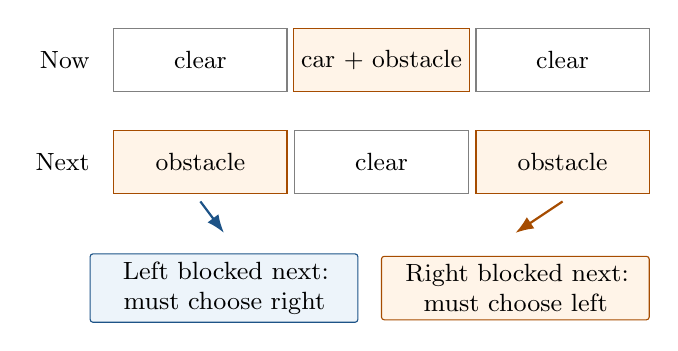
\begin{tikzpicture}[x=1mm,y=1mm,>=Latex,
every node/.style={font=\small,align=center,inner sep=1mm},
cell/.style={draw=black!50,minimum width=22mm,minimum height=8mm},
blocked/.style={cell,draw=fliporange,fill=softorange}]
\node[anchor=east] at (15,32) {Now};
\node[cell] at (28,32) {clear};
\node[blocked] at (51,32) {car + obstacle};
\node[cell] at (74,32) {clear};
\node[anchor=east] at (15,19) {Next};
\node[blocked] at (28,19) {obstacle};
\node[cell] at (51,19) {clear};
\node[blocked] at (74,19) {obstacle};
\node[draw=sourceblue,fill=softblue,text width=32mm,rounded corners=1pt]
 at (31,3) {Left blocked next:\\must choose right};
\node[draw=fliporange,fill=softorange,text width=32mm,rounded corners=1pt]
 at (68,3) {Right blocked next:\\must choose left};
\draw[->,thick,sourceblue] (28,14)--(31,10);
\draw[->,thick,fliporange] (74,14)--(68,10);
\end{tikzpicture}
\caption{Vehicle's first-change conflict. Both outer lanes blocked next
is source-forbidden but helper-legal. The current middle obstacle activates
both response rules, so no single next lane satisfies them.}
\label{fig:vehicle-first-change}
\end{figure}


The source can win from this state. A source-legal next input leaves an
obstacle-free outer lane. Choose it. Thereafter obey the forced lane moves;
otherwise choose an obstacle-free middle lane. If the middle is blocked,
stay in the current outer lane or move from the middle to an outer lane. Set speed to one when the selected lane has a green
light, no pedestrian and no obstacle, and to zero otherwise. After the first
response the policy selects the middle whenever that lane is free, so its
recurring availability implies the recurring free-lane goal.
Supplement~E supplies the invariant, all speed duties and full proof.

For \emph{each} saved source winner, including each loss, there exists an
initialized Kind strategy and a compatible source-legal play reaching that
target at time one. Both may depend on the target: this is neither a common
controller nor forced reachability. Supplements~X and AD.3 give the
target-specific predecessor and all-history completion proofs. No update,
public Kind query or replacement execution was performed for Vehicle.

\subsection{Obstacle: can one first-change duty alter a solver answer?}
At exact query B, releasing that duty changes the fixed raw answer from
false to true. Unlike Patrol's later loss of an initially available response,
Obstacle has an immediate first-change obstruction at every state. It tests
the implementation consequence and the effect of releasing the duty.

The published Obstacle Evasion old/update pair~\cite{dupdate} changes
forbidden locations and recurring SYS visit goals. We consider two exact
queries, each fixing its input specification and initializer. A uses the old source and its authored initializer. B uses the
updated ordinary projection---the source with only the parse-time switch
declaration removed---and fixes a retained point: obstacle $(3,5)$,
\code{obsWait=true}, robot $(5,5)$. A uses obstacle $(7,7)$,
\code{obsWait=false}, robot $(1,1)$. Each query has one ENV initial value
and the specified SYS response; the full universal-ENV/existential-SYS
initial obligation is retained. B's point was fixed by a seven-edge legal
prefix in the old winning region before computing the new region. The old
initializer is not conjoined. This is full requirements replacement,
not an ENV-only update or preservation of the old pending goals.

\paragraph{Both exact queries have source-kind witnesses}
Each direct-source certificate alternates between two goal phases; for B
these mean visiting $(3,7)$ and $(4,8)$, with a finite nonnegative rank that
is zero exactly at the current goal. A separately implemented checker
enumerates every legal ENV input and checks the supplied response for full
SYS safety and closure within the certified states, strict rank decrease with unchanged phase away from
the goal, and a phase switch at the goal, where no rank decrease is required.
It also checks the full initial quantifiers: the accepted certificates
establish a winning strategy for each exact query, not a maximal region.
The ENV relation is independent of the next SYS response, total on all
6,272 typed states, and has no justice assumptions. Consequently every
history of a typed-total completion of the strict witness admits an ENV-safe,
fair suffix using that same strategy and reached memory. Both exact queries
therefore have source-kind witnesses (Supplement~AC.5--AC.7).

What a negative tool answer says about those witnesses depends on the
comparison. Table~\ref{tab:obstacle-comparisons} keeps the three experiments
separate.

\begin{table}[!ht]
\caption{Three completed Obstacle comparisons: fixed-strict regions,
public-mode answers and the exact-B raw intervention.
The separate exported-game audit group has eight UNKNOWNs.}
\label{tab:obstacle-comparisons}\centering\small
\begin{tabular}{@{}L{18mm}L{29mm}L{33mm}@{}}\toprule
Question & Procedure / change & Result\\\midrule
Strict survival & Fixed strict solver; source + three helper games & Release and correction recover source regions.\\[4pt]
Public answer & Ordinary vs Kind; translation and solver change & Ordinary: true; Kind: false (A, B).\\[4pt]
Raw effect at B & Fixed cooperative solver; duty kept $\to$ released & False $\to$ true.\\\bottomrule
\end{tabular}
\end{table}


\paragraph{Release and correction recover both strict source regions}
Table~\ref{tab:obstacle-regions} gives the completed comparison under the
same released strict GR1Game solver, with source requirements and types fixed.
The syntactic helper loses every strict source winner. These are strict
regions, not cooperative regions returned by the public Kind procedure.
Source avoidance excludes the current robot from the next obstacle footprint.
On a first helper change a typed input can place the footprint over that
robot, regardless of its response. Export relation checks bind this
obstruction to both syntactic games. First-change release removes the SYS duty only on the $0\to1$ quadrant;
complete correction guards the whole SYS relation. Both recover the source regions state by state.
These exports have $U=D$.

\begin{table}[!ht]
\caption{Completed fixed strict-solver comparison: winning-state counts.
The update region has no initializer; exact point query B is separate.}
\label{tab:obstacle-regions}\centering\small
\begin{tabular}{@{}lrr@{}}\toprule
Game & Old & Update\\\midrule
Source & 5,016 & 5,015\\
Syntactic helper, $b=0$ & 0 & 0\\
First-change release, $b=0$ & 5,016 & 5,015\\
Complete correction, $b=0$ & 5,016 & 5,015\\\bottomrule
\end{tabular}
\end{table}

The old query retains its authored initializer. B's point lies in the recovered
update region and its singleton initial quantifiers give the corresponding
strict conclusion. This fixed-strict comparison completed two source and
six translated native queries (Supplement~AC.2--AC.4).

\paragraph{Public ordinary mode is positive and Kind mode negative}
For each of A and B, the public ordinary-GR(1) action returned true and the
Kind action false, once per mode under the same release and backend
settings. Mode selection changes \emph{both} translation and solver, so
this comparison alone does not isolate a cause. Code and console records
identify a static syntactic-reduction/raw-solver path, separate from the
complete correction. A was already negative before the update
(Supplement~AE).

\paragraph{Releasing one duty changes the raw answer at B}
At exact B, two fresh processes called the same cooperative four-fixed-point
raw solver and completed normally: unchanged returned \textbf{false};
first-change release returned \textbf{true}. Input and initializer checks
bind the source certificate and separate ENV-totality result to both raw
arms' source query, with the helper initially false.
With translation/backend settings fixed, typed comparisons verify all other
relations, domains, initializers and ordered justices unchanged; quadrant
differences verify complete SYS release only on typed $0\to1$, with typed
$1\to1$ already true. Supplement~AG records this local intervention and
execution protocol; AF retains the separate earlier false/UNKNOWN protocol.

If used as a continuation gate at B, the public Kind negative would reject
the source-kind witness above. The raw pair establishes a local intervention
effect; exclusion still requires the query-and-objective correspondence below.

\subsection{Cohort: which losses are ruled out by the certified sample?}
\label{sec:cohort}
The cohort asks where loss can be ruled out, rather than how often it occurs.
Loss of all-history source-kind winners is excluded in 58 models for the
\emph{literal strict target}, although ten models have strict-state losses.
The remaining model's exact cooperative-loss intersection is UNKNOWN.
Table~\ref{tab:cohort} shows the complete 49/9/1 partition.

Here \emph{legal-prefix cooperation} means that after every source-legal
prefix induced by one strict-winning strategy, that same strategy at its
reached memory permits an ENV-safe, fair continuation. All-history
source-kind winners form a subset, because they also require cooperation
after violations.
\begin{table}[!ht]
\caption{Stopped, completion-and-certificate-conditioned cohort.
The preservation target is the complete literal strict encoding.}
\label{tab:cohort}\centering\small
\begin{tabular}{@{}rL{69mm}@{}}\toprule
Models & Established outcome\\\midrule
49 & Entire strict source-winning region preserved.\\[3pt]
9 & Strict-state losses occur, but no legal-prefix cooperative source winner is lost.\\[3pt]
1 & Strict loss is known; the exact cooperative-loss intersection remains UNKNOWN (corpus159, RoboticArm).\\\bottomrule
\end{tabular}
\end{table}

No cooperative-initialization loss is confirmed. Of 425 public units,
70 completed and 59 remained after eleven certification exclusions, without
outcome filtering within the eligible set. All three cases lie outside this
stopped cohort. Completion and certification conditioning preclude an
incidence or rarity estimate for operational Kind/update states or public
actions. Supplement~AB.5 records case selection and Patrol277's certificate
exclusion, which its later proof does not undo.

\FloatBarrier
\section{Auditing Candidate Exclusion}\label{sec:discussion}
\subsection{An exclusion contract}
In replacement planning, a negative answer can exclude a source continuation only when the query,
translation and answering procedure support that inference. The result gives
an implementer's reasoning contract with three steps.

\paragraph{Fix the query and objective}
Decide whether the question is about a retained state or about all allowed
initial ENV values and their selectable SYS responses. Also distinguish strict
winning from a cooperation requirement such as Kind. For a retained entry,
fields and pending monitors are part of the state. Initial realizability
cannot substitute for this query, and installing a particular controller
additionally requires compatible private memory.

\paragraph{Establish preservation for that query}
Check that the actual translation has the required typed relations, auxiliary
updates, initializers and ordered justices. For a fixed retained state $s$,
preservation means $s\in W\Rightarrow s\in W_C$, or
$s\in W\Rightarrow s\in W_F$ under retained duties
(Theorem~\ref{hpb:exact} and Proposition~\ref{hpb:retained}). A strategy may
leave a queried set and must still maintain its response option; immediate
responses alone are insufficient.

With unchanged initializers and initial $b=0$, initialized strict synthesis
instead compares the $\forall$ENV$\exists$SYS initial decisions. For an
initially realizable source, the decision is preserved exactly when every
allowed ENV initial value admits at least one allowed SYS response in $W_C$
(or $W_F$). It need not preserve every winning initial response. Source
initial unrealizability is already preserved by $W_C,W_F\subseteq W$.

Whole-region preservation holds exactly when $W\subseteq C$ or
$W\subseteq F$. This is sufficient, but generally not necessary, for
initial-decision preservation. Checking these conditions can require game solving; no inexpensive online
test is implied.

\paragraph{Establish what the negative answer rules out}
With the corresponding preservation obligation, a sound negative
\emph{strict} answer rules out the source property queried: winning from
the fixed retained state, or initialized realizability. A public Kind procedure
has a different intended objective; its negative answer needs its own
correspondence to that source objective. Our strict theorem does not supply
it.

To rule out source-kind existence, it suffices that such existence imply
a positive encoded strict answer for the same retained state or initial
quantifiers. Preserving all strict source winners is therefore conservative.
Missing preservation or correspondence means exclusion lacks support;
that is neither a positive source result nor a solver UNKNOWN.

Patrol gives the concrete obstruction: a positive source query lies outside
$W_F$, so its encoded strict negative cannot exclude it. Obstacle adds a
source-kind positive premise and negative public answer, with a local
answer-changing intervention at B. That intervention does not replace the
query-and-objective correspondence required by the contract.

\subsection{Inspecting the accompanying artifact}\label{sec:artifact}
The accompanying release~\cite{artifactrepository} provides three checks.
Vehicle checks saved loss membership and target-specific predecessors.
Patrol checks the positive policy, all-response countercertificate and typed
export premises. Obstacle B checks the shared query and sole SYS release
behind the positive witness and raw false/true pair.
The supplement reader guide and artifact reading map give the
detailed tasks and evidence locations.

These checks reuse saved native results and case certificates; file integrity
and document source closure remain separate from scientific replay.

\section{Scope and Relation to Prior Work}\label{sec:scope}
\subsection{Limits shared by the cases}
The cases and conditioned cohort do not estimate operational incidence.
Positive certificates establish existence, not maximality, while saved-region
comparisons share native-solver, exporter and type-metadata dependencies;
the case checks independently validate neither saved-region maximality
nor the compiler. The exact-B intervention does not reconstruct a historical
GUI game or establish a corrected public pipeline, controller extraction
or transfer.

The Patrol execution discussed here reused its legal policy without gate
mediation or new controller installation. Supplements~U.4 and U.9 separately
record bounded software-adapter admission and installation; they do not
implement the exclusion contract above. The off-assumption
completion is not a physical recovery demonstration. Existence does not
transfer arbitrary old-controller memory. We assume prepared candidate
requirements and a valid hold of the retained entry; a changed state needs
a verified update bridge or revalidation before installation. Inspection
cost, benefit over direct source solving, gate/installation benefit and
performance advantages remain open.

\subsection{Relation to prior work}\label{sec:related}
Adaptation methods construct choices: multi-tier control prepares alternatives,
exploration discovers environment behavior, and weakening, degradation and
recovery change requirements~\cite{dippolito2014multitier,keegan2022discovery,weakening2023,graceful2024}.
Interpolation and permissive assumptions refine admissible ENV
behavior~\cite{cavezza2017interpolation,anand2023apa}.
Our characterization addresses a different step: when a translated negative
answer justifies excluding a source continuation from those choices.

Dynamic-update synthesis constructs controller
bridges~\cite{nahabedian2020dynamic,dupdate}; runtime verification retains
monitors across requirement changes~\cite{runtimeverification2023}.
These works explain why reached states and pending obligations matter.
Preservation is a condition to establish before using an encoded negative
to reject a candidate for such a bridge or installation.

Cooperative synthesis, well-separation and best-effort GR(1) address
assumption handling and fairness opportunities~\cite{cooperative,friendly,wellsep,besteffort}.
Kind adds an all-history condition~\cite{kind}; we establish that positive
source premise separately from strict-region preservation. Extraction has
additional hypotheses: IROS constrains middle-fixed-point choices
\cite[author appendix, p.~9]{iros}, while acceleration assumes language
inclusion~\cite[Secs.~2.3,~4.1]{accelerating}. We do not derive those guarantees
from the preservation theorem.

Earlier GR(1) work studies preprocessing false negatives, completeness
conditions and a correction~\cite{klein2011revisiting}, distinguishing
implication and strict realizability. Our source and encoded games both use
strict semantics; the existing helper correction and our preservation
contribution are distinguished in Section~\ref{sec:intro}.

\section{Conclusion}\label{sec:conclusion}
A safe response now does not ensure that a winning continuation survives a
one-way helper encoding. The exact condition is that one source-winning
strategy can maintain the first-change response option; with retained duties,
that response must enter a region that remains safe. Patrol demonstrates the
difference at one retained entry with a positive policy and an argument covering
all safe strategies. Vehicle and Obstacle connect preservation to distinct
initialization and tool queries, including the controlled false-to-true result
at exact B. Together with executable case checks, the characterization makes
the justification for candidate exclusion explicit and inspectable.

\section*{Acknowledgments}
We used OpenAI Codex~\cite{codex} and Anthropic Claude Code in refining
this research. Their assistance included experiment design, derivation,
implementation, execution, auditing and analysis. These internal AI reviews
are not human review or proof-assistant verification. The public artifact~\cite{artifactrepository}
records the workflow and evidence scope underlying the checks reported in
this study.
\begin{thebibliography}{25}
\interlinepenalty=0
\clubpenalty=0
\widowpenalty=0
\bibitem{autonomic2003}J. O. Kephart and D. M. Chess, ``The vision of autonomic computing,'' \emph{Computer}, vol. 36, no. 1, pp. 41--50, Jan. 2003. doi: \href{https://doi.org/10.1109/MC.2003.1160055}{10.1109/MC.2003.1160055}.
\bibitem{specrepair}T. Buckworth, D. Alrajeh, J. Kramer, and S. Uchitel, ``Adapting specifications for reactive controllers,'' in \emph{SEAMS}, 2023, pp. 1--12. doi: \href{https://doi.org/10.1109/SEAMS59076.2023.00012}{10.1109/SEAMS59076.2023.00012}.
\bibitem{degradation}T.-A. Georgescu, D. Alrajeh, and S. Uchitel, ``Learning to adapt GR(1) specifications through degradation,'' arXiv:2609.12231v1, Sept. 2026. \url{https://arxiv.org/abs/2609.12231v1}.
\bibitem{dupdate}G. Amram, S. Maoz, I. Segall, and M. Yossef, ``Dynamic update for synthesized GR(1) controllers,'' in \emph{ICSE}, 2022, pp. 786--797. doi: \href{https://doi.org/10.1145/3510003.3510054}{10.1145/3510003.3510054}.
\bibitem{kind}A. Gorenstein, S. Maoz, and J. O. Ringert, ``Kind controllers and fast heuristics for non-well-separated GR(1) specifications,'' in \emph{ICSE}, 2024. doi: \href{https://doi.org/10.1145/3597503.3608131}{10.1145/3597503.3608131}.
\bibitem{spectrarelease2024}Software Modeling Lab, ``Spectra Tools: Released Game-Model Bundle,'' version 1.0.0.202402072123, 2024. Bundled source: \code{PitermanSemanticReduction}. \url{https://smlab.cs.tau.ac.il/syntech/spectra/tools/update/plugins/tau.smlab.syntech.gamemodel_1.0.0.202402072123.jar}.
\bibitem{artifactrepository} Anonymous artifact contributors, \emph{Controller Replacement Audit: Accompanying Artifact and Paper Reading Map}, v71-r10, Oct. 2026. \url{https://github.com/research-artifact-archive/seams2027/blob/controller-replacement-audit-20261026-v10/paper/README.md}.
\bibitem{gr1}R. Bloem, B. Jobstmann, N. Piterman, A. Pnueli, and Y. Sa'ar, ``Synthesis of Reactive(1) Designs,'' \emph{J. Comput. Syst. Sci.}, vol. 78, no. 3, pp. 911--938, 2012. doi: \href{https://doi.org/10.1016/j.jcss.2011.08.007}{10.1016/j.jcss.2011.08.007}.
\bibitem{kindartifact}A. Gorenstein, S. Maoz, and J. O. Ringert, ``Artifact for ICSE'24 paper: Kind Controllers and Fast Heuristics for Non-Well-Separated GR(1) Specifications,'' Zenodo, v3, 2024. doi: \href{https://doi.org/10.5281/zenodo.10553249}{10.5281/zenodo.10553249}.
\bibitem{cooperative}R. Bloem, R. Ehlers, and R. K\"onighofer, ``Cooperative reactive synthesis,'' in \emph{ATVA}, 2015, pp. 394--410. doi: \href{https://doi.org/10.1007/978-3-319-24953-7_29}{10.1007/978-3-319-24953-7\_29}.
\bibitem{friendly}R. Majumdar, N. Piterman, and A.-K. Schmuck, ``Environmentally-friendly GR(1) synthesis,'' in \emph{TACAS}, 2019, pp. 229--246. doi: \href{https://doi.org/10.1007/978-3-030-17465-1_13}{10.1007/978-3-030-17465-1\_13}. Extended proofs: \url{https://arxiv.org/abs/1902.05629}.
\bibitem{vehicleartifact}Anonymous, \emph{Vehicle188 Native Strict Evidence}, version vehicle188-native-evidence-20261024-v1, Oct.~2026. \url{https://github.com/research-artifact-archive/seams2027/blob/vehicle188-native-evidence-20261024-v1/VEHICLE188_NATIVE_EVIDENCE.md}.
\bibitem{spectra}S. Maoz and J. O. Ringert, ``Spectra: a specification language for reactive systems,'' \emph{Software and Systems Modeling}, vol. 20, pp. 1553--1586, 2021. doi: \href{https://doi.org/10.1007/s10270-021-00868-z}{10.1007/s10270-021-00868-z}.
\bibitem{vehiclewholeartifact}Anonymous artifact contributors, \emph{Vehicle188 whole-region saved evidence}, version vehicle188-whole-region-evidence-20261024-v1, Oct.~2026. \url{https://github.com/research-artifact-archive/seams2027/blob/vehicle188-whole-region-evidence-20261024-v1/VEHICLE188_WHOLE_REGION_EVIDENCE.md}.
\bibitem{dippolito2014multitier}N. D'Ippolito, V. Braberman, J. Kramer, J. Magee, D. Sykes, and S. Uchitel, ``Hope for the best, prepare for the worst: Multi-tier control for adaptive systems,'' in \emph{ICSE}, 2014, pp. 688--699. doi: \href{https://doi.org/10.1145/2568225.2568264}{10.1145/2568225.2568264}.
\bibitem{keegan2022discovery}M. Keegan, V. Braberman, N. D'Ippolito, N. Piterman, and S. Uchitel, ``Control and discovery of environment behaviour,'' \emph{IEEE Transactions on Software Engineering}, vol. 48, no. 6, pp. 1965--1978, 2022. doi: \href{https://doi.org/10.1109/TSE.2020.3044532}{10.1109/TSE.2020.3044532}.
\bibitem{weakening2023}S. Chu, E. Shedden, C. Zhang, R. Meira-G\'oes, G. A. Moreno, D. Garlan, and E. Kang, ``Runtime resolution of feature interactions through adaptive requirement weakening,'' in \emph{SEAMS}, 2023, pp. 115--125. doi: \href{https://doi.org/10.1109/SEAMS59076.2023.00025}{10.1109/SEAMS59076.2023.00025}.
\bibitem{graceful2024}S. Chu, J. Koe, D. Garlan, and E. Kang, ``Integrating graceful degradation and recovery through requirement-driven adaptation,'' in \emph{SEAMS}, 2024, pp. 122--132. doi: \href{https://doi.org/10.1145/3643915.3644090}{10.1145/3643915.3644090}.
\bibitem{cavezza2017interpolation}D. G. Cavezza and D. Alrajeh, ``Interpolation-based GR(1) assumptions refinement,'' in \emph{TACAS}, 2017, pp. 281--297. doi: \href{https://doi.org/10.1007/978-3-662-54577-5_16}{10.1007/978-3-662-54577-5\_16}.
\bibitem{anand2023apa}A. Anand, K. Mallik, S. P. Nayak, and A.-K. Schmuck, ``Computing adequately permissive assumptions for synthesis,'' in \emph{TACAS}, 2023, pp. 211--228. doi: \href{https://doi.org/10.1007/978-3-031-30820-8_15}{10.1007/978-3-031-30820-8\_15}.
\bibitem{nahabedian2020dynamic}L. Nahabedian, V. Braberman, N. D'Ippolito, S. Honiden, J. Kramer, K. Tei, and S. Uchitel, ``Dynamic update of discrete event controllers,'' \emph{IEEE Transactions on Software Engineering}, vol. 46, no. 11, pp. 1220--1240, 2020. doi: \href{https://doi.org/10.1109/TSE.2018.2876843}{10.1109/TSE.2018.2876843}.
\bibitem{runtimeverification2023}M. Carwehl, T. Vogel, G. N. Rodrigues, and L. Grunske, ``Runtime verification of self-adaptive systems with changing requirements,'' in \emph{SEAMS}, 2023, pp. 104--114. doi: \href{https://doi.org/10.1109/SEAMS59076.2023.00024}{10.1109/SEAMS59076.2023.00024}.
\bibitem{wellsep}S. Maoz and J. O. Ringert, ``On well-separation of GR(1) specifications,'' in \emph{FSE}, 2016, pp. 362--372. doi: \href{https://doi.org/10.1145/2950290.2950300}{10.1145/2950290.2950300}.
\bibitem{besteffort}S. Liu, Y. Zhang, C. Hu, and W. Dong, ``Best-effort GR(1) synthesis: Exploiting environmental cooperation under unrealizability,'' in \emph{ASE}, 2026, pp. 1806--1818. doi: \href{https://doi.org/10.1145/3832783.3837439}{10.1145/3832783.3837439}.
\bibitem{iros}R. Ehlers, R. K\"onighofer, and R. Bloem, ``Synthesizing cooperative reactive mission plans,'' in \emph{IEEE/RSJ International Conference on Intelligent Robots and Systems (IROS)}, 2015, pp. 3478--3485. doi: \href{https://doi.org/10.1109/IROS.2015.7353862}{10.1109/IROS.2015.7353862}. Author version with appendix: \url{https://www.ruediger-ehlers.de/papers/iros2015.pdf}.
\bibitem{accelerating}S. Liu and W. Dong, ``Accelerating kind realizability: A multi-stage incremental realizability checking framework,'' in \emph{FM}, 2026, pp. 240--258. doi: \href{https://doi.org/10.1007/978-3-032-26204-2_13}{10.1007/978-3-032-26204-2\_13}.
\bibitem{klein2011revisiting}U. Klein and A. Pnueli, ``Revisiting synthesis of GR(1) specifications,'' in \emph{Hardware and Software: Verification and Testing (HVC 2010)}, LNCS 6504, 2011, pp. 161--181. doi: \href{https://doi.org/10.1007/978-3-642-19583-9_16}{10.1007/978-3-642-19583-9\_16}.
\bibitem{codex}OpenAI, \emph{Codex}, 2026. Accessed Oct.~23, 2026. \url{https://openai.com/codex/}.
\bibitem{claudecode}Anthropic, \emph{Claude Code}, 2026. Accessed Oct.~26, 2026. \url{https://claude.com/product/claude-code}.
\end{thebibliography}

\end{document}
